% !TEX TS-program = pdflatex
% !TEX encoding = UTF-8 Unicode
%
% MODIFIED by Nathan Baker, 2011-03-23
% Added PNNL colors
%
% MODIFIED by Jonathan Kew, 2008-07-06
% The header comments and encoding in this file were modified for inclusion with TeXworks.
% The content is otherwise unchanged from the original distributed with the beamer package.
%
% CREATED by Till Tantau <tantau@users.sourceforge.net>, 2004

\documentclass{beamer}

\mode<presentation>
{

	% AnnArbor
	% 	Overrides PNNL color scheme
	% Antibes (header outline)
	% 	Personal favorite
	% 	Use of colors is a bit busy
	% Bergen
	% 	Does something strange -- colors look brown
	% 	Avoid using
	% Berkeley (sidebar outline)
	% 	Logo doesn't work
	% Berlin (header outline)
	% 	Header text might be too faint
	% Boadilla
	% 	OK but not very aesthetically pleasing
	% 	Footer can get crowded
	% CambridgeUS
	% 	Partially overrides PNNL color scheme
	% Copenhagen
	% 	OK; could make better use of secondary/tertiary/quaternary colors
	% Darmstadt
	% 	Nice progress bar on top
	% 	Cross-faded header is a bit strange
	% Dresden
	% 	Looks washed out
	% Frankfurt (header outline)
	% 	Nice progress bar
	% 	Personal favorite when progress bar is needed
	% Goettingen (sidebar outline)
	% 	A mess; sidebar color is ugly
	% Hannover (sidebar outline)
	% 	Meh.
	% Ilmenau
	% 	Questionable color arrangement
	% JuanLesPins
	% 	See ``Darmstadt'' comments
	% 	Ugly numbers and bullets
	% Luebeck (header outline)
	% 	Could make better use of secondary/tertiary colors
	% Madrid
	% 	See ``Boadilla'' comments
	% 	Ugly numbers and bullets
	% Malmoe (header outline)
	% 	Personal favorite
	% Marburg (sidebar outline)
	% 	Overrides PNNL colors
	% Montpellier
	% 	Looks really bad
	% PaloAlto
	% 	Logo is fouled up
	% Pittsburgh
	% 	Minimal
	% 	Personal favorite
	% Rochester
	% 	Looks a lot like one of the PNNL PPT templates
	% 	Personal favorite
	% Singapore
	% 	Washed out
	% Szeged
	% 	Ugly
	% Warsaw
	% 	Cross-fade from orange to gray is strange
	% boxes
	% 	Looks like minimal PNNL PPT template
	% 	Personal favorite
	% default
	% 	Looks like minimal PNNL PPT template
	% 	Personal favorite
	\usetheme{Malmoe}
	% \setbeamercovered{transparent}
	
	% Colors based on http://brand.pnl.gov/guide/color.aspx
	\definecolor{PNNLorange}{RGB}{213,117,0}
	\definecolor{PNNLgray}{RGB}{112,114,118}
	\definecolor{PNNLbronze}{RGB}{255,160,35}
	\definecolor{PNNLgold}{RGB}{241,171,0}
	\definecolor{PNNLonyx}{RGB}{36,36,36}
	\definecolor{PNNLplatinum}{RGB}{178,179,181}

	% Define colors for use
	% abstract
	% abstract title
	% alerted text
	\setbeamercolor{alerted text}{fg=PNNLbronze}
	% author
	\setbeamercolor{author}{fg=PNNLonyx}
	% author in head/foot
	\setbeamercolor{author in head/foot}{bg=PNNLgray}
	% author in sidebar
	% background
	% background canvas
	% bibliography entry author
	% bibliography entry location
	% bibliography entry note
	% bibliography entry title
	% bibliography item
	% block body
	% block body alerted
	% block body example
	% block title
	% block title alerted
	% block title example
	% button
	% button border
	% caption
	% caption name
	% date
	\setbeamercolor{date}{fg=PNNLgray}
	% date in head/foot
	% date in sidebar
	% description item
	% enumerate item
	% enumerate subitem
	% enumerate subsubitem
	% example text
	\setbeamercolor{example text}{fg=PNNLonyx}
	% fine separation line
	% footline
	% framesubtitle
	% frametitle
	% frametitle right
	% headline
	% institute
	% institute in head/foot
	% institute in sidebar
	% item
	% item projected
	% itemize item
	% itemize subitem
	% itemize subsubitem
	% itemize/enumerate body
	% itemize/enumerate subbody
	% itemize/enumerate subsubbody
	% local structure
	% logo
	% lower separation line foot
	% lower separation line head
	% math text
	% math text displayed
	% math text inlined
	% middle separation line foot
	% middle separation line head
	% mini frame
	% navigation symbols
	% navigation symbols dimmed
	% normal text
	\setbeamercolor{normal text}{fg=PNNLonyx}
	% normal text in math text
	% normal text in math text
	% page number in head/foot
	% palette primary
	\setbeamercolor{palette primary}{bg=PNNLorange}
	% palette quaternary
	\setbeamercolor{palette quaternary}{bg=PNNLgray}
	% palette secondary
	\setbeamercolor{palette secondary}{bg=PNNLgold}
	% palette sidebar primary
	% palette sidebar quaternary
	% palette sidebar secondary
	% palette sidebar tertiary
	\setbeamercolor{palette tertiary}{bg=PNNLbronze}
	% palette tertiary
	% part name
	% part title
	% qed symbol
	% quotation
	% quote
	% section in head/foot
	% section in sidebar
	% section in sidebar shaded
	% section in toc
	% section in toc shaded
	% section name
	% section number projected
	% section title
	% separation line
	% sidebar
	% sidebar left
	% sidebar right
	% structure
	\setbeamercolor{structure}{fg=PNNLorange}
	% subitem
	% subitem projected
	% subsection in head/foot
	% subsection in sidebar
	% subsection in sidebar shaded
	% subsection in toc
	% subsection in toc shaded
	% subsection name
	% subsection number projected
	% subsection title
	% subsubitem
	% subsubitem projected
	% subsubsection in head/foot
	% subsubsection in sidebar
	% subsubsection in sidebar shaded
	% subsubsection in toc
	% subsubsection in toc shaded
	% subsubsection number projected
	% subtitle
	% title
	% title in head/foot
	% title in sidebar
	% titlegraphic
	% titlelike
	% upper separation line foot
	% upper separation line head
	% verse

	% Fun with fonts
	\usefonttheme{default}
	\useinnertheme{default}
	\useoutertheme{infolines}
	\setbeamerfont{author}{size=\large}
	\setbeamerfont{date}{size=\large}
	\setbeamerfont{example text}{series=\bfseries}
	\setbeamerfont{frametitle}{series=\bfseries,size=\large}
	\setbeamerfont{framesubtitle}{series=\mdseries,size=\large}
	\setbeamerfont{section}{series=\bfseries}
	\setbeamerfont{title}{series=\bfseries}

	% Navigation controls
	\setbeamertemplate{navigation symbols}{}
	
	% Logo on every page
	\logo{
	    
\includegraphics[height=1cm]{img/umd_logo.png}
        \hspace*{.55\paperwidth}
        \includegraphics[height=1cm]{img/pnnl_logo.jpg}
    }
}


\usepackage[english]{babel}
% or whatever

\usepackage[utf8]{inputenc}
% or whatever

%\usepackage{times}
%\usepackage[T1]{fontenc}
% Or whatever. Note that the encoding and the font should match. If T1
% does not look nice, try deleting the line with the fontenc.

\usepackage[ruled]{algorithm2e}
\usepackage{algorithmic}
\usepackage{bbm}
\usepackage{caption}
\usepackage{subcaption}

\newcommand{\R}{{\mathbb{R}}}
\newcommand{\bbP}{{\mathbb{P}}}
\newcommand{\bbI}{{\mathbbm{1}}}

\newtheorem*{remark}{Remark}

\title[Optimal Transport for Super Resolution] % (optional, use only with long paper titles)
{Optimal Transport for Super Resolution Applied to Astronomy Imaging}

\author[Rawson, Hultgren] % (optional, use only with lots of authors)
{Michael G. Rawson\inst{1,2}, 
Jakob Hultgren\inst{2}
}

\institute[] % (optional, but mostly needed)
{
  \inst{1}%
  Pacific Northwest National Laboratory, Seattle, WA, USA \\
  \inst{2}
  University of Maryland at College Park, College Park, MD, USA
}
% - Use the \inst command only if there are several affiliations.
% - Keep it simple, no one is interested in your street address.

\date[] % (optional)
{July 15, 2022}

%\subject{Talks}
% This is only inserted into the PDF information catalog. Can be left
% out.

% If you have a file called "university-logo-filename.xxx", where xxx
% is a graphic format that can be processed by latex or pdflatex,
% resp., then you can add a logo as follows:

% \pgfdeclareimage[height=0.5cm]{university-logo}{university-logo-filename}
% \logo{\pgfuseimage{university-logo}}



% Delete this, if you do not want the table of contents to pop up at
% the beginning of each subsection:

% \AtBeginSection[]
% {
% 	\begin{frame}<beamer>{Outline}
% 	\small
% 	\tableofcontents[currentsection,currentsubsection]
%   \end{frame}
% }



% If you wish to uncover everything in a step-wise fashion, uncomment
% the following command:

%\beamerdefaultoverlayspecification{<+->}


\begin{document}

\begin{frame}
	\titlepage
\end{frame}

\begin{frame}
    \frametitle{Contents}
    \begin{minipage}{\textwidth}
    \tableofcontents       
    \end{minipage}
\end{frame}

\section{Introduction}

% \subsection{Super Resolution}

\begin{frame}{Super Resolution}
    Super resolution seeks to improve image resolution without further data collection.
    \pause
    
    ~
    
    This is possible, given constraints that give a well-posed inverse problem, for example smoothness or \textbf{sparsity}.
    \pause
    
    ~
    
    \centerline{\includegraphics[width=.5\textwidth]{img/Super resolution.jpg}}
    
    
\end{frame}

% \subsection{Optimal Transport}

\begin{frame}{Optimal Transport}
    \begin{definition}
    Let $\mu\in\mathbb R^n_{\ge 0}, \nu \in \mathbb R^m_{\ge 0}$ be probability vectors and $C\in \mathbb R^n\times \mathbb R^m$.     
    \pause
    Then the optimal transport plan from $\mu$ to $\nu$ is                            
\begin{equation} 
    \arg\min_{P\in \Pi(\mu,\nu)} \sum_{i=1}^n \sum_{j=1}^n C_{ij} P_{ij} 
\end{equation}
\pause
where 
$ \Pi(\mu,\nu) = \{P\in\mathbb R^{n\times m}: \sum_{i=1}^n P_{ij} = \nu_j\ \forall j, \sum_{j=1}^n P_{ij} = \mu_i\ \forall i\}. $
    \end{definition}
    \centerline{\includegraphics[width=.5\textwidth]{img/Optimal Transport.jpg}}
\end{frame}

% \subsection{Entropy}

\begin{frame}{Entropy}
\pause
    \begin{definition}
    For a probability mass function $p:\mathcal J\rightarrow \mathbb R$ (non-negative and sums to 1), we will use $H(p)$ to denote its entropy,
\begin{equation} 
    H(p) = -\sum_{\iota \in \mathcal J} p(\iota) \ln(p(\iota)) \label{eq:Entropy}. 
\end{equation}
    \end{definition}
    \pause
    \textbf{Key point:} Sparse arrays have low entropy. 
\end{frame}

% \subsection{Sinkhorn Algorithm}

\begin{frame}{Entropic regularisation}
    Approximate optimal transport distances can be computed by solving the entropic regularization of optimal transport
    $$ \arg\min_{P\in \Pi(\mu,\nu)} \sum_{i=1}^n \sum_{j=1}^n C_{ij}P_{ij} - \epsilon H(P). $$
    \pause
    
    ~
    
    This is equivalent to the matrix scaling problem, more precisely finding positive multipliers $f\in \mathbb R^n, g\in \mathbb R^m$ such that the matrix
    $$ (f_i e^{-C_{ij}/\epsilon} g_j) \in \Pi(\mu,\nu). $$

\end{frame}

% \subsection{Wasserstein Distance Gradient}

\begin{frame}{Sinkhorn}
    The matrix scaling problem can be solved with the Sinkhorn algorithm, alternating between solving 
    $$\sum_{j=1}^m f_i e^{-C_{ij}/\epsilon} g_j = \mu_i$$ 
    for $f$ 
    \pause 
    and then solving 
    $$ \sum_{i=1}^n f_i e^{-C_{ij}/\epsilon} g_j = \nu_j $$
    for $g$. 
    
\end{frame}

\begin{frame}{Wasserstein Distance Gradient}
    The multipliers $f$ and $g$ play the role of Lagrange multipliers and can be used to approximate the variation of $W(\mu,\nu)$ with respect to the first and second argument respectively. 
    \pause
    
    ~
    
    This can be used to implement gradient descent methods. 
\end{frame}

\section{Wasserstein Inverse Problem}

\begin{frame}{Wasserstein Inverse Problem for Super Resolution}
\vspace{-5ex}
    For a measurement $\nu$ and positive regularization parameter $\lambda$, we define the \emph{sparse approximation} of $\nu$ as a minimizer 
\begin{equation}
    \mu_* = \arg\min_{\mu \in \bbP(X)} d_W^\epsilon(\mu,\nu) + \lambda H(\mu).
    \label{eq:sparseNeigh}
\end{equation}
\vspace{-4ex}
\small
\pause
\begin{itemize}
    \item At least one minimizer exists by compactness of the finite dimensional probability simplex. 
\pause
    \item The entropy term favors sparse solutions. There is a trade-off between sparsity of the solution and proximity to the measurement. 
\pause
    \item This inverse problem is useful whenever there is a natural distance, or cost function, on the index set of $\nu$. 
\pause
    \item We will let each entry in $\nu$ describe the intensity of a pixel in a $32\times 32$ image and cost $C_{ij}$ is chosen as the $L^2$-distance between the $i^{th}$ pixel and $j^{th}$ pixel.
\end{itemize}

\end{frame}

\section{Algorithm}

\subsection{Sinkhorn Gradient}

\begin{frame}{}
\small

\textbf{Input:} 
$\mu, \nu \in \R^n$ : positive probability vectors,
$C\in\R^{n \times n}$ : cost matrix,
$\epsilon$ : positive regularization parameter

\pause
\textbf{Output:}
$d_W^\epsilon \in \R$ : regularized distance between $\mu$ and $\nu$,
$F \in \R^n$ : gradient of $d_W^\epsilon(\mu,\nu)$ with resp. to $\mu$ at $\mu$,
$G \in \R^n$ : gradient of $d_W^\epsilon(\mu,\nu)$ with resp. to $\nu$ at $\nu$
\pause

\hfill
\begin{minipage}{.74\textwidth}
\begin{algorithm}[H]
    
    % \textbf{Begin:} 

    $f = (1,\ldots,1)\in \R^n$
    
    $g = (1,\ldots,1)\in \R^n$
    
	\While{$f$ and $g$ have not converged}
 	{
 	    \For{$1 \le i \le n$}{
     	$f_i = \mu_i / \left(\sum_j \exp(-C_{ij}/\epsilon) g_j\right)$ 
     	}\pause
     	\For{$1 \le j \le n$}{
     	$g_j = \nu_j / \left(\sum_i \exp(-C_{ij}/\epsilon) f_i\right)$ 
     	}
  	}
  	\pause

    $d_W^\epsilon = \sum_{i=1}^n \sum_{j=1}^n f_i g_j \exp(-C_{ij} /\epsilon) C_{ij}$ 
  	
  	$F = -\epsilon \ln(f)$
  	
  	$G = -\epsilon \ln(g)$\\
  	
	\caption{ The Sinkhorn Algorithm for Optimal Transport Distances}
	\label{algo:Sinkhorn}
\end{algorithm}
\end{minipage}

\end{frame}

\subsection{Super Resolution}

\begin{frame}{}
\small

    \textbf{Input:} 
     $X \in \R^{N \times m \times m}$ : $N$ images size $m \times m$,
     $\lambda \in \R$ : positive noise level,
     $0 < \epsilon < 1$ : optimal transportation regularization,
     $C\in\R^{m^2 \times m^2}$ : cost matrix,
     $ J_{\lambda,\epsilon}(x,v) := d_W^\epsilon(x,v) + \lambda H(v) $
\pause

    \textbf{Output:}
     $K \in \R^N$ : star cluster classification
\pause

\hfill
\begin{minipage}{.74\textwidth}
\begin{algorithm}[H]
    
    % \textbf{Begin:}
    
    $K = 0$
    
	\For{$i=1,2,...,N$}
 	{
% $ V_i = \arg\min_{v} d_W^\epsilon(X_n,v) + \lambda H(v)$\\
        $ v = X_i $ \\
    	\While{ $v$ has not converged }
 	    {
$w = \nabla d_W^\epsilon(X_i,\cdot)|_v + \lambda \nabla H|_v $ \\
$ w = w - \langle w, \frac{1}{m} \bbI \rangle \cdot \frac{1}{m} \bbI $ \\
\pause
$ \alpha = \sup\{\alpha \in \R : J_{\lambda,\epsilon}(v) > J_{\lambda,\epsilon}(v - \alpha w) \}$ \\
            $ \alpha = \min\{0.01, \alpha\}$\\
\pause
 	        $ v = v - \alpha w $;
 	        $ v = diag(\bbI_{v > 0}) \ v $;
 	        $ v = v/\|v\|_1 $
 	    }
\pause
 	    $V_i = v$;
     	$\delta = \max V_i$
     	
        \If{ $rank(H_0(V_i^{-1}([0.75 \delta,\ \delta]))) == 1$ }{ 
            $ K_i = 1 $ 
        }
  	}
	\caption{\tiny O.T. Super Resolution Clustering \cite{rawson_astro}}
	\label{algo:star_cluster}
\end{algorithm}
\end{minipage}

\end{frame}


\section{Theoretic Results}

\subsection{Optimal Transport Bound on Gaussian Noise}

\begin{frame}{Optimal Transport Bound on Gaussian Noise}
\begin{theorem}[\cite{rawson_astro}]
Let $\nu = \frac{1}{k}\sum_{i=1}^k \delta_{p_i}$ where $p_i\in \mathbb R^d$ and $\tilde\nu$ be the noisy signal acquired by sampling, for each $i$, $n$ points according to a normal distribution centered at $p_i$ with independent components of variance $\sigma^2$. \pause
Then the Wasserstein distance between $\nu$ and $\bar\nu$ is bounded by a random variable with expected value $d\sigma^2$ and variance $2d\sigma^4/N$,  where $N=nk$ is the total number of points sampled.  
\end{theorem}
\pause

\centerline{\includegraphics[width=.6\textwidth]{img/Gaussian.jpg}}

\end{frame}

\subsection{Reconstructing the Support of a Sparse Signal}

\begin{frame}{Reconstructing the Support of a Sparse Signal}

\begin{theorem}[\cite{rawson_astro}]
    \label{thm1}
    Assume $\nu$ is a sparse signal and $\bar\nu$ is a noisy signal such that 
    $d_w(\nu,\bar\nu) < \delta $. \pause
    Then the solution of 
    \begin{equation*} \label{eq:dualConstraint} 
        \mu=\arg\min_{\mu : d_W(\bar\nu,\mu) \le \delta} H(\mu) 
    \end{equation*} 
    will identify the structure of $\mu$, i.e. have the same support as $\mu$, if $||\nu||_0 \leq ||\mu||_0$ for all $\mu$ such that $d_W(\mu,\bar\nu)<2\delta$, with equality only if $\mu$ and $\nu$ has the same support.  
\end{theorem}

\end{frame}

\begin{frame}{Reconstructing the Support of a Sparse Signal \cite{rawson_astro}}

\vspace{-5ex}

\begin{remark}
    The conditions in Theorem~\ref{thm1} can be summarized as a low enough noise level $\delta$ and enough sparsity of the true signal $\nu$ (making it a local minimizer of the $L^0$-norm). \pause
    It is interesting to note that these conditions are essentially necessary: if the inequality in Theorem~\ref{thm1} is violated by some $\mu$ closer than $\delta$ to $\bar\nu$, then the solution of \eqref{eq:dualConstraint} does not identify the structure of $\nu$. 
\end{remark}
\pause

\begin{remark}
    Noise is high entropy, hence it is expected that the noise can be removed by minimizing the entropy. \pause
    However, if the signal-to-noise ratio is too low, this reconstruction is underdetermined.
\end{remark}

\end{frame}

\begin{frame}{Reconstructing the Support of a Sparse Signal}

\begin{theorem}[\cite{rawson_astro}]
    Fix a positive probability vector $\nu\in\R^d_{>0}$ such that all elements of $\nu$ are distinct. 
    \pause
    Then the sparse recovery is continuous to perturbations around $\nu$ for small $\lambda$, i.e. for every $\epsilon'>0$ there exists $\delta>0$, such that 
    if $d_W(\nu,\nu')<\delta$,
    $\mu_* = \arg\min_{\mu \in \bbP(X) : d_W(\mu, \nu)<\lambda} H(\mu)$,
    and 
    $\mu_*' = \arg\min_{\mu \in \bbP(X) : d_W(\mu, \nu')<\lambda} H(\mu)$
    \pause
    then $\|\mu_*-\mu_*'\| < \epsilon'.$
    \label{thm:robust}
\end{theorem}

\end{frame}


\section{Numerical Results}

\subsection{Simulation}

\begin{frame}{Let measurement $ \hat\nu = (0.2, 0.15, 0, 0, 0, 0.1, 0.15, 0.2, 0.15, 0.1) $ }
\pause
\vspace{-5ex}
\begin{figure}
\centering
\begin{subfigure}[b]{0.45\textwidth}
\centering
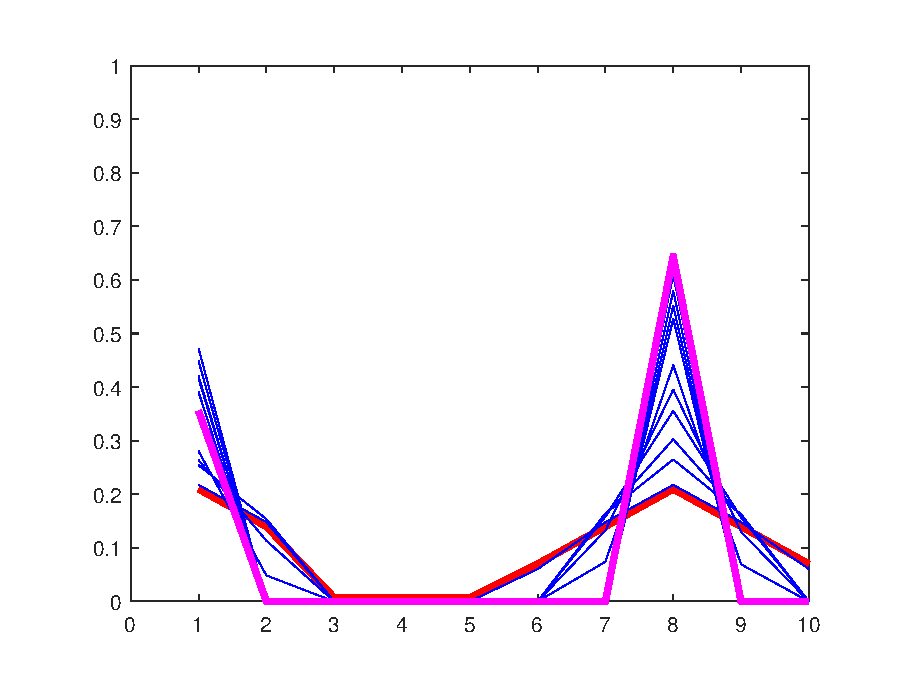
\includegraphics[width=1.1\textwidth]{img/OT_gradient_descent_1D_lambda=10.eps}
\caption{Sparsity level $\lambda=10$. Solution $ \nu = (0.35,0,0,0,0,0,0,0.65,0,0)$. }
\label{fig:low_sparse}
\end{subfigure}
% \hfill
\pause
\begin{subfigure}[b]{0.45\textwidth}
\centering
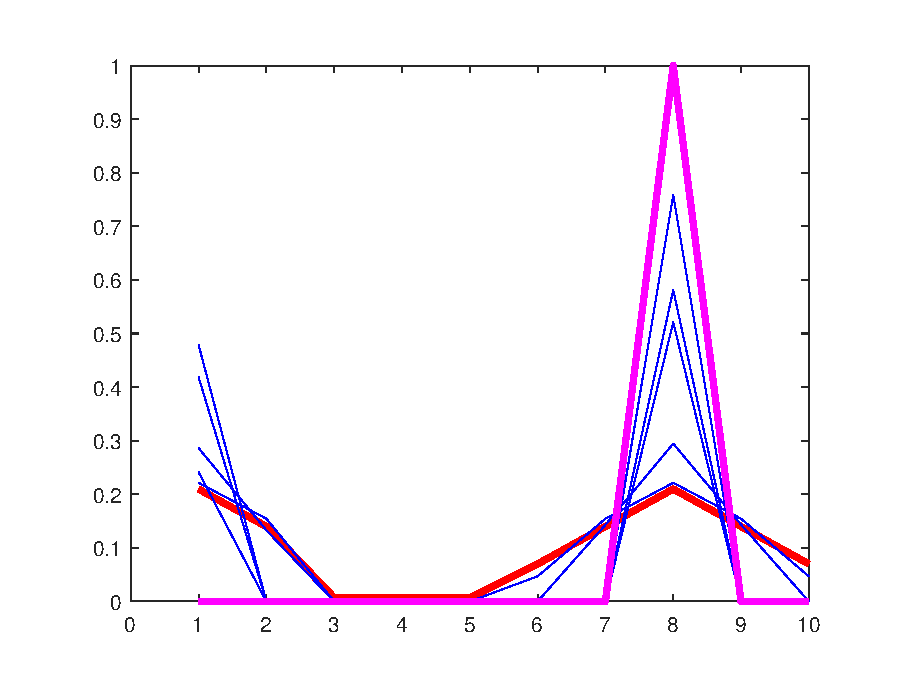
\includegraphics[width=1.1\textwidth]{img/OT_gradient_descent_1D_lambda=100.eps}
\caption{Sparsity level $\lambda=100$. Solution $\nu = (0,0,0,0,0,0,0,1,0,0)$.}
\label{fig:high_sparse}
\end{subfigure}
\caption{Plot of super resolution O.T. method. Red line is initial distribution. Blue lines are steps along gradient. Pink line is final, converged distribution.}
\end{figure}

\end{frame}

\subsection{Star Clustering Application}

\begin{frame}{Star Clustering Application}

\begin{itemize}
    \item The formation and evolution of star clusters \cite{perez_starcnet_2021} \pause
    \item Algorithmically detect star clusters in images of sky patches \pause
    \item State of the art method trains a convolutional neural network (CNN) to classify each region in an image as containing a star cluster or not \cite{perez_starcnet_2021} \pause
    \item Neural networks are notoriously computationally expensive, sensitive to noise, and inflexible to appending or removing data variables
\end{itemize}

\end{frame}

\begin{frame}{Star Clustering Application \cite{rawson_astro}}
\vspace{-6ex}
\begin{table}
\caption{Confusion matrix of O.T. method on LEGUS data compared to StarcNet \cite{perez_starcnet_2021}. Column gives StarcNet classification and row gives O.T. classification \cite{rawson_astro}.}
\begin{center}
\begin{tabular}{c|c|c|}
 & StarcNet Cluster & StarcNet Not Cluster \\
\hline
O.T. Cluster     & 25\% (32) & 13.3\% (17)  \\
\hline
O.T. Not Cluster & 12.5\% (16) & 49.2\% (63)  \\
\hline
\end{tabular}
\label{table:2}
\end{center}
\end{table}
\small
 \pause
 \begin{itemize}
    \item The accuracy rate of clustering without sparsifying is 46\% w.r.t. the CNN.  \pause
    \item The O.T. method increases in accuracy to 74\% with respect to the CNN.  \pause
    \item The CNN accuracy rate is 86\% with respect to experts, but even experts agree with each other only around 70\%-75\% \cite{ wei_deep_2020}.  \pause
    \item Our method provides a very high performance given that no neural network training, which often takes weeks of compute time, is required. 
\end{itemize}

\end{frame}

\section{Conclusion}

\begin{frame}{Conclusion}
\begin{itemize}
    \item 
Optimal transportation is more 
\begin{itemize}
    \item efficient,  \pause
    \item robust,  \pause
    \item flexible  
\end{itemize}
than CNNs. \pause
\item We proved that optimal transportation will reconstruct sparse sources and is robust to noise
\item Relevant for correcting distortions and noise in imaging, ex: star cluster detection
\item A predictive model for star clusters can produce a \emph{policy} that informs where future surveys should look for star clusters \cite{rawson_deep_2021, freeman}. 

\end{itemize}

\end{frame}

\begin{frame}{End}
\begin{center}    
    Thank You!
    
    ~
    
    Questions?

    ~

    michael.rawson@pnnl.gov, hultgren@umd.edu
    
\end{center}

\end{frame}

\begin{frame}{References}
\tiny
    \bibliographystyle{apalike}
    \bibliography{ref.bib}
\end{frame}

\end{document}


